\documentclass[a4paper, 13pt]{article}
% \usepackage{vntex}
%\usepackage[english,vietnam]{babel}
%\usepackage[utf8]{inputenc}

%\usepackage[utf8]{inputenc}
%\usepackage[francais]{babel}
\usepackage{a4wide,amssymb,epsfig,latexsym,multicol,array,hhline,fancyhdr}
\usepackage{booktabs}
\usepackage{amsmath}
\usepackage{setspace}
\usepackage{longtable}
\usepackage{lastpage}
\usepackage[lined,boxed,commentsnumbered]{algorithm2e}
\usepackage{enumerate}
\usepackage{color, colortbl}
\usepackage{graphicx}							% Standard graphics package
\usepackage{array}
\usepackage{tabularx, caption}
\usepackage{multirow}
\usepackage[framemethod=tikz]{mdframed}% For highlighting paragraph backgrounds
\usepackage{multicol}
\usepackage{rotating}
\usepackage{graphics}
\usepackage{geometry}
\usepackage{setspace}
\usepackage{epsfig}
\usepackage{tikz,lipsum,lmodern}
\usepackage[most]{tcolorbox}
\usepackage{array}
\usepackage{float}
\newcommand{\PreserveBackslash}[1]{\let\temp=\\#1\let\\=\temp}
\newcolumntype{C}[1]{>{\PreserveBackslash\centering}p{#1}}
\newcolumntype{R}[1]{>{\PreserveBackslash\raggedleft}p{#1}}
\newcolumntype{L}[1]{>{\PreserveBackslash\raggedright}p{#1}}
\usepackage{listings}
\usetikzlibrary{arrows,snakes,backgrounds}
\usepackage{hyperref}
\hypersetup{urlcolor=blue,linkcolor=black,citecolor=black,colorlinks=true} 
%\usepackage{pstcol} 								% PSTricks with the standard color package
\renewcommand{\arraystretch}{1.5}

% \newtheorem{theorem}{{\bf Định lý}}
% \newtheorem{property}{{\bf Tính chất}}
% \newtheorem{proposition}{{\bf Mệnh đề}}
% \newtheorem{corollary}[proposition]{{\bf Hệ quả}}
% \newtheorem{lemma}[proposition]{{\bf Bổ đề}}

% \everymath{\color{red}}
%\usepackage{fancyhdr}
\setlength{\headheight}{40pt}
\pagestyle{fancy}
\fancyhead{} % clear all header fields
\fancyhead[L]{
 \begin{tabular}{rl}
    \begin{picture}(25,15)(0,0)
    \put(0,-8){\includegraphics[width=8mm, height=8mm]{hcmut.png}}
    %\put(0,-8){\epsfig{width=10mm,figure=hcmut.eps}}
   \end{picture}&
	%\includegraphics[width=8mm, height=8mm]{hcmut.png} & %
	\begin{tabular}{l}
		\textbf{\bf \ttfamily Ho Chi Minh University of Technology}\\
		\textbf{\bf \ttfamily Faculty of Computer Science and Engineering}
	\end{tabular} 	
 \end{tabular}
}
\fancyhead[R]{
	\begin{tabular}{l}
		\tiny \bf \\
		\tiny \bf 
	\end{tabular}  }
\fancyfoot{} % clear all footer fields
\fancyfoot[L]{\scriptsize \ttfamily Software Engineering Assignment - Academic Year 2022-2023}
\fancyfoot[R]{\scriptsize \ttfamily Page {\thepage}/\pageref{LastPage}}
\renewcommand{\headrulewidth}{0.3pt}
\renewcommand{\footrulewidth}{0.3pt}

%%%
\setcounter{secnumdepth}{4}
\setcounter{tocdepth}{3}
\makeatletter
\newcounter {subsubsubsection}[subsubsection]
\renewcommand\thesubsubsubsection{\thesubsubsection .\@alph\c@subsubsubsection}
\newcommand\subsubsubsection{\@startsection{subsubsubsection}{4}{\z@}%
                                     {-3.25ex\@plus -1ex \@minus -.2ex}%
                                     {1.5ex \@plus .2ex}%
                                     {\normalfont\normalsize\bfseries}}
\newcommand*\l@subsubsubsection{\@dottedtocline{3}{10.0em}{4.1em}}
\newcommand*{\subsubsubsectionmark}[1]{}
\makeatother

\definecolor{dkgreen}{rgb}{0,0.6,0}
\definecolor{gray}{rgb}{0.5,0.5,0.5}
\definecolor{mauve}{rgb}{0.58,0,0.82}
\definecolor{LightCyan}{rgb}{0.88,1,1}
\definecolor{moccasin}{rgb}{0.98, 0.92, 0.84}

\lstset{frame=tb,
	language=Matlab,
	aboveskip=3mm,
	belowskip=3mm,
	showstringspaces=false,
	columns=flexible,
	basicstyle={\small\ttfamily},
	numbers=none,
	numberstyle=\tiny\color{gray},
	keywordstyle=\color{blue},
	commentstyle=\color{dkgreen},
	stringstyle=\color{mauve},
	breaklines=true,
	breakatwhitespace=true,
	tabsize=3,
	numbers=left,
	stepnumber=1,
	numbersep=1pt,    
	firstnumber=1,
	numberfirstline=true
}

\begin{document}

\begin{titlepage}
\begin{center}
Vietnam National University - Ho Chi Minh City \\
Ho Chi Minh City University of Technology \\
Faculty of Computer Science and Engineering \\
Department of Software Engineering 
\end{center}

\vspace{1cm}

\begin{figure}[h!]
\begin{center}
\includegraphics[width=3cm]{hcmut.png}
\end{center}
\end{figure}

\vspace{1cm}


\begin{center}
\begin{tabular}{c}
	\multicolumn{1}{l}{\textbf{{\Large Software Engineering Capstone Project }}}\\
	~~\\
	\hline
	\\
	%\multicolumn{1}{l}{\textbf{{\Large Software Development}}}\\
	\\
	
	\textbf{{\Huge Urban Waste Collection Aid 2.0}}\\
	\\
	\hline
\end{tabular}
\end{center}

\vspace{3cm}

\begin{table}[h]
\begin{tabular}{rrl}
\hspace{5 cm} & Instructor: &Dr. Truong Tuan Anh\\
& Student: & Tran Le Trung Chanh - 2052403\\
& &  Nguyen Khanh Duy  - 2052425\\
& & Nguyen Minh Hoang - 2052481\\
& & Duong Ngoc Quang Huy - 2052489\\
& & Nguyen Ho Quang - 2052666\\
\end{tabular}
\end{table}

\begin{center}
{\footnotesize Ho Chi Minh, 09/2022}
\end{center}
\end{titlepage}
\onehalfspacing
\tableofcontents
\newpage
\listoffigures
\newpage
\listoftables
\newpage

\section{Introduction}
The Sustainable Development Goals (SDGs), adopted by United Nations Members in 2015, are a shared blueprint for peace and prosperity for people and the planet, now and into the future. These goals are an urgent call for action for all countries, with an emphasis on strategies that focus on improving health and education, reducing inequality, and spurring economic growth – all while tackling climate change and working to preserve our oceans and forests. Which, particular attention is given to SDG 11: sustainable cities and communities and SDG 6: clean water and sanitation for developing countries. With these goals in mind, we take a look at an urban context, where the solid waste management system yields low results while progressively increase in costs. As an example, currently, in Vietnam, the waste management system is still operated manually with assigned collectors. These collectors are usually assigned to a specific route or a specific area without any consideration for fuel economy or traffic. As a result, the system is proven to be costly and time-consuming. Therefore, our project will be revolving around improving the current waste collection and management system using techniques in the domain of Computer Science.

\section{TASK\#1}

\subsection{Problem Statement}
\begin{tcolorbox}[colback=blue!5!white,colframe=blue!75!black]
  In this section, we will represent the context of this project as well as the relevant stakeholders. We also explain their current needs and some problem facing. In the end, we state our opinion on the benefits that UWC 2.0 will deliver to each stakeholder.
\end{tcolorbox}

\subsubsection{Context of the project}

In the context of this project, we were provided with a working waste managing system called Urban Waste Collection Aid - UWC: Janitors will take responsibility for gathering the garbage in a small neighbourhood and bring it manually to the major collecting points (MCPs). Collectors will have a specific route to come through the major collecting points and pick up the garbage. Calendar and routes given to teams of janitors and collectors will be coordinated by Back officers. There should be a strong communication line between the back officers and teams of janitors and collectors via messaging. In addition, the system already has a database, consisting of information from version 1.0 of UWC. We will be developing the 2.0 version of UWC, which is contracted to Organization X from Service Provider Y, to improve the efficiency of garbage collection and implement the Task Assignment Module provided in the assignment.
\newpage

\subsubsection{Relevant Stakeholders}
\begin{itemize}
    \item Back officers
    \item Janitors
    \item Collectors
    \item Organization X
    \item Service Provider Y
\end{itemize}
\subsubsection{Current needs \& problems}
\textbf{User story} \\
Traditionally, a collecting team of at least two members, one janitor and one collector, will be assigned to a small area, where they take round trips around that area to collect waste house by house. Janitors want to gather around the neighbourhood quickly and then he will bring it to a specific place for his partner to collect. Collectors want to pick up one time and drive to other collecting points so that they can finish their job faster. Usually, the route is fixed and the truck stop house by house for one person to load up the truck. This system while simple introduces some problems regarding the efficiency and time consumption of the system. Without prior planning, the route might be hard to commute or closed for certain times, therefore, the collector has to waste time in traffic or have to take another route, which. As a result, we recommend a new position - back officers, this position will be able to access an overview of the whole system, including but not limited to collectors, janitors as well as other resources. Based on that information, the back officers should be able to schedule and assign tasks to teams of collectors and janitors effectively. In this project specifically, the back officers have to take into consideration some requirements about the fuel consumption and distance of travel of the vehicles to create and optimize the path taken by the collectors, with clear communication to the teams. In addition, these assignments and tasks will be stored in a database, together with other data from the staff, which can be accessed by a system administrator to be used for further analysis, an example would be to forecast the tasks based on historical analogies.\\
\newpage
\textbf{Needs \& problems}
%chắc là vẽ thêm bảng need + problems cho đẹp

\begin{longtable}{|p{0.2\textwidth}|p{0.35\textwidth}|p{0.35\textwidth}|} 
\hline
    \textbf{Stakeholders} & \textbf{Needs} & \textbf{Problems} \\

\hline
Back officers & A platform to assign tasks and communicate with teams of janitors and collectors, view information on available resources & No communications between teams. Cannot assign tasks to teams. Have no view of available resources\\
\hline
Janitors & Being able to receive assigned tasks  &  \\
\hline 
Collectors & Being able to receive assigned routes & \\
\hline 
Organization X & Build a suitable solution & Build UWC 2.0 with the specify requirements \\
\hline 
Service Provider Y & An improved version of UWC & Improve the system and upgrade and import the old database from UWC 1.0\\
\hline 
    \caption{Stakeholder's need and problem}
\end{longtable}

\subsubsection{Benefits}
In our opinion, UWC 2.0 offers many benefits to the stakeholders. For instance, the back officers will be provided with a functional platform for administrative tasks, which promises better performance, quicker response time, and more direct communication via messages between teams. From the perspective of collectors and janitors, their tasks should be more straightforward and less time-consuming, improving productivity. \\
To service provider Y, the project introduces many solutions to both current and future issues. An example would be increasing the efficiency of the system by reducing the number of active vehicles and teams or yielding better results in fewer working hours. The data collected might also be instrumental in future developments. \\
All in all, UWC 2.0 is a suitable automation solution the current waste management system, pushing the industry to a digital future.
\\
\subsection{Functional Requirements}
\begin{tcolorbox}[colback=blue!5!white,colframe=blue!75!black]
  In this section, we will represent some functional requirements of the whole system in general and the specific requirements of the operation of back officers. For the ease of referring to particular requirements, we attached each requirement and its group with an identification. Therefore, we can further refer to the identification given to get the function group name or specific requirement description.
\end{tcolorbox}
\subsubsubsection*{General Requirements}
\begin{longtable}{|p{0.25\textwidth}|p{0.7\textwidth}|} 
    \hline
         \textbf{Requirement Identification (ID)} & \textbf{Requirement Description} \\
         \hline 
         \endfirsthead
         
         \hline
        \caption{Functional requirements for the general operation of the whole system} \\
         \endlastfoot

         \hline
         \multicolumn{2}{l}{Continued from the previous page.}
         \hline
          Requirement Identification (ID) & Requirement Description \\
          \hline
          \endhead

          \hline
         \multicolumn{2}{r}{Continued on the next page \ldots}\\
         \hline
        \endfoot
        
         \rowcolor{moccasin} \textbf{F01} & \textbf{Register} \\
         \hline
         F01\_01 &  Users can register with an available valid username and password \\
         \hline
         F01\_02 &  The system can catch and display any error messages in registering an account \\
         \hline
         F01\_03 &  The system can save the account information (username, password, etc.) in the database \\
         \hline
         %%%%%%%%%%%%%%%%%%%%%%%%%%%%%
         \rowcolor{moccasin} \textbf{F02} & \textbf{Login} \\
         \hline
         F02\_01 &  Users can log in to the system by the registered account \\ 
                  \hline
         F02\_02 &  The system can catch and display any error messages in logging in \\
         \hline
         %%%%%%%%%%%%%%%%%%%%%%%%%%%%%%%%%%%%%%%%%%%%%%
         \rowcolor{moccasin} \textbf{F03} & \textbf{Display} \\
         \hline
         F03\_01 &  The system can display the information of janitors and collectors \\
         \hline
         F03\_02 &  The system can display the work calendar of janitor teams and collectors \\         \hline

         F03\_03 &  The system can display the details of vehicles such as weight, capacity, fuel consumption, etc \\         \hline

         F03\_04 &  The system can display the information of all MCPs such as location, capacity, etc \\         \hline

         F03\_05 &  The system can display the tracking information of each collector \\
         \hline
         F03\_06 & The system has language switching setting \\
         \hline
         %%%%%%%%%%%%%%%%%%%%%%%%%%%%%%%%%%%%%%%%%%%
         \rowcolor{moccasin} \textbf{F04} & \flushcenter{\textbf{Logout}} \\
         \hline
         F04\_01 &  Users can log out of the system \\
         \hline
         %%%%%%%%%%%%%%%%%%%%%%%%%%%%%%%%%%%%%%%%%%
         \rowcolor{moccasin} \textbf{F05} & \textbf{Communication} \\
         \hline
         F05\_01 &  Back officers can communicate with janitors and collectors via messages \\
         \hline
         F05\_02 &  Janitors and collectors can communicate via messages \\
         \hline
         %%%%%%%%%%%%%%%%%%%%%%%%%%%%%%%%%%%%%%%5
         \rowcolor{moccasin} \textbf{F06} & \textbf{Update information} \\
         \hline
         F06\_01 &  Users can change/update personal information as well as password \\
         \hline
          F06\_01 &  The ongoing status of each user should be updated to the system \\
         \hline
         %%%%%%%%%%%%%%%%%%%%%%%%%%%%%%%%%%%%%%%%%%%%%%%%
         \rowcolor{moccasin} \textbf{F07} & \textbf{Security} \\
         \hline
         F07\_01 &  The system can verify the long-term inactive user \\
         \hline
         F07\_02 &  Backup \\
         \hline
    \end{longtable}   
\newpage
\subsubsubsection*{Back Officiers Requirements}
\begin{table}[h]
    \centering
    \begin{tabular}{| p{0.25\textwidth} | p{0.7\textwidth}|} 
    \hline
         Requirement Identification (ID) & Requirement Description \\
         \hline 
         \rowcolor{moccasin} \textbf{F08} & \textbf{Assignment} \\
         \hline
         F08\_01 &  The system provides an interface for back officers to assign vehicles to janitors and collectors \\
         \hline
         F08\_02 &  The system provides an interface for back officers to assign janitors and collectors to MCPs \\
         \hline
         F08\_03 &  The system provides an interface for creating routes to MCPs \\
         \hline
         %%%%%%%%%%%%%%%%%%%%%%%%%%%%%
         %%%%%%%%%%%%%%%%%%%%%%%%%%%%%%%%%%%%%%%%%%%
         \end{tabular}
    \caption{Functional requirements for the operation of back officiers}
    \label{tab:my_label}
\end{table}
\subsection{Non-functional Requirements}
\begin{tcolorbox}[colback=blue!5!white,colframe=blue!75!black]
  In this section, we will represent the non-functional requirements of the system.
\end{tcolorbox}
\subsubsubsection*{Non-functional requirements}
\begin{longtable}{|p{0.25\textwidth}|p{0.7\textwidth}|} 
    \hline
         
         \textbf{Requirement Identification (ID)} & \textbf{Requirement Description} \\
         \hline 
         \endfirsthead
         
         \hline
        \caption{Non-functional requirements of the whole system categorized into several criterion} \\
         \endlastfoot

         \hline
         \multicolumn{2}{l}{Continued from the previous page.}
         \hline
          Requirement Identification (ID) & Requirement Description \\
          \hline
          \endhead

          \hline
         \multicolumn{2}{r}{Continued on the next page \ldots}\\
         \hline
        \endfoot
        
         \rowcolor{moccasin} \textbf{NF01} & \textbf{Operation} \\
         \hline
         NF01\_01 &  The system should be accessible from any device with a stable internet connection \\
         \hline
         
         NF01\_02 &  The system has a user friendly interface \\
         \hline
          NF01\_03 &  Information should be updated from MCPs every 15 minutes with the availability of at least 95\% of their operating time \\
         \hline
          NF01\_04 &  The system has an interchangeable language setting (Vietnamese - English) \\
         \hline
          NF01\_05 &  Information of tasks on a daily and weekly basis must be displayed in one view \\
         \hline
         %%%%%%%%%%%%%%%%%%%%%%%%%%%%%
         \rowcolor{moccasin} \textbf{NF02} & \textbf{Performance} \\
         \hline
         NF02\_01 &  The system can be accessed at any time (24h/day 365 days/per year) \\ 
                  \hline
         NF02\_02 &  Assigned route is optimized in terms of fuel consumption and travel distance \\
         \hline
         NF02\_03 &  Messages are sent with less than a 1-second delay \\
         \hline
         %%%%%%%%%%%%%%%%%%%%%%%%%%%%%%%%%%%%%%%%%%%%%%
         \rowcolor{moccasin} \textbf{NF03} & \textbf{Security} \\
         \hline
         NF03\_01 &  The system can be accessed with the registered username and password \\
         \hline
         NF03\_02 &  Meet basic cybersecurity standards (Authentication, Authorization, Data Protection) \\         \hline

         NF03\_03 &  Cooldown time when login failed more than 3 times \\         \hline
         %%%%%%%%%%%%%%%%%%%%%%%%%%%%%%%%%%%%%%%%%%%
         \rowcolor{moccasin} \textbf{NF04} & \textbf{External} \\
         \hline
         NF04\_01 &  The system must comply with the law of the host government \\
         \hline
         NF04\_02 &  The system must guarantee that information of a certain employee is private\\
         \hline
         
    \end{longtable} 
    
\newpage
\subsection{Use-case Diagram}
\begin{tcolorbox}[colback=blue!5!white,colframe=blue!75!black]
  In this section, we will represent the use-case study via use-case diagrams of the whole system and task assignment module. We also include the relation between the use cases.
\end{tcolorbox}
\subsubsection*{Use-case diagram of a whole system}
\begin{center}
    \begin{figure}
        \centering
        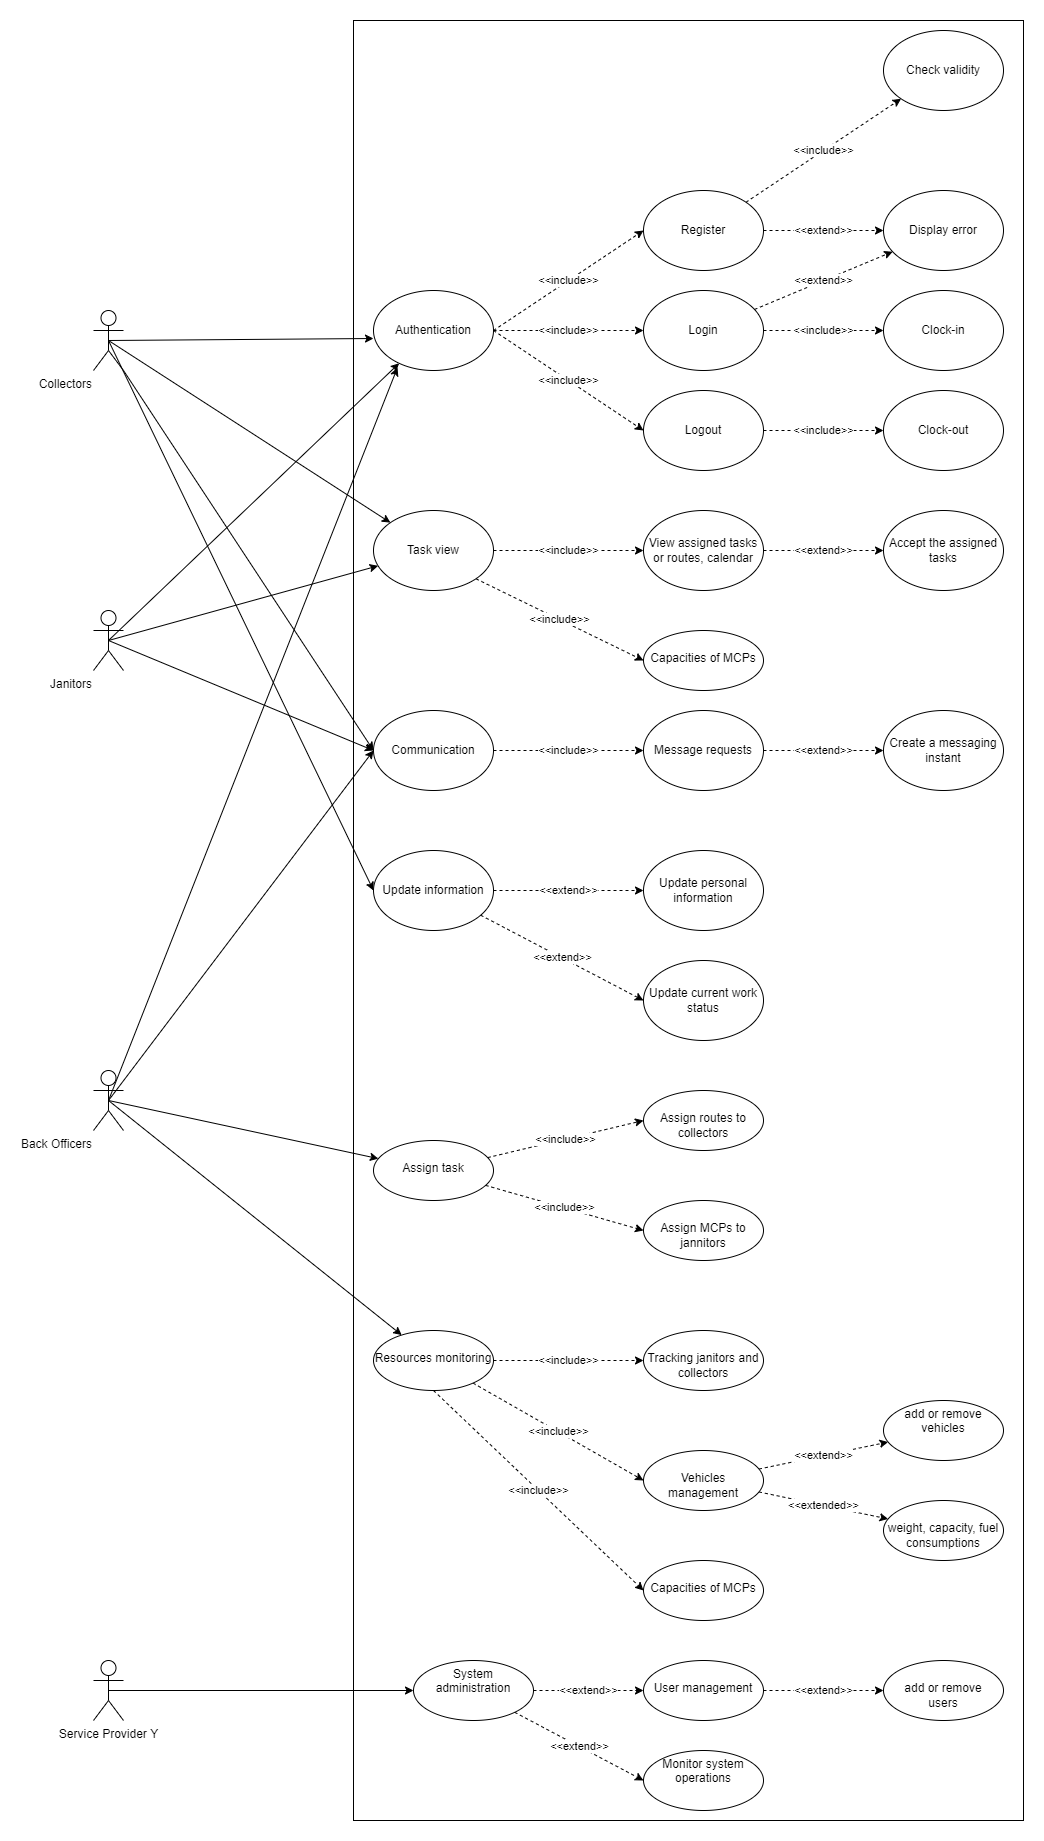
\includegraphics[scale=0.3]{requirement/systemUC.png}
        \caption{UWC 2.0}
        \label{fig:my_label}
    \end{figure}
\end{center}
\subsubsection*{Use-case diagram of the task assign module}

\begin{figure}[H]
    \centering
    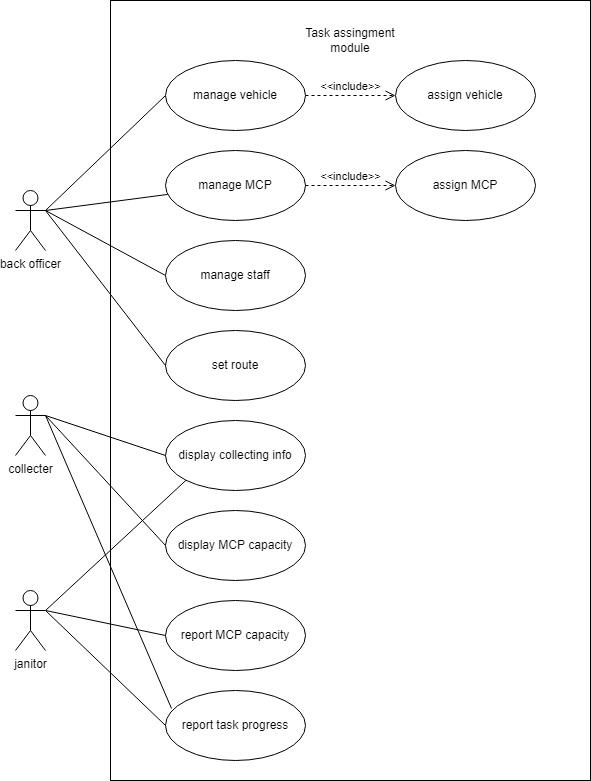
\includegraphics[scale=0.6]{requirement/assignModule.jpg}
    \caption{Task Assignment module}
    \label{fig:my_label}
\end{figure}
\newpage
\subsubsection*{Use-case table}
\begin{longtable}{|p{0.25\textwidth}|p{0.7\textwidth}|} 
    
         \multicolumn{2}{c}{Use-case table - Task assign module} \\
         \hline 
         \endfirsthead
         
         \hline
        \caption{Use-case table explaining the diagram of the task assign module} \\
         \endlastfoot

         \hline
         \multicolumn{2}{l}{Continued from the previous page.}
         \hline
          
          \endhead

          \hline
         \multicolumn{2}{r}{Continued on the next page \ldots}\\
         \hline
        \endfoot

        Use case ID & UC\_01 \\
        Use case name & Manage vehicle \\
        Description & View all information of the available vehicle, including capacity, weight, fuel consumption, etc.\\
        Actors & Back officer, database\\
        Trigger & Select the manage vehicle option\\
        Pre-condition & Have access to internet, the database is available for update\\
        Post-condition & Back officer has an overview of the vehicles\\
        Step & 1.~Select the manage vehicle option\\
         & 2.~Show all the available vehicles and their technical details\\
        Exception & \\
    
        \rowcolor{moccasin} & &

        %%%%%%%%%%%%%%%%%%%% U2
        Use case ID & UC\_02 \\
        Use case name & Assign vehicle \\
        Description & Assign appropriate vehicle for collector base on their collecting route\\
        Actors & Back officer, database\\
        Trigger & Select the vehicle assigning option\\
        Pre-condition & Have access to internet, the database is available for update\\
        Post-condition & Each collector get assigned to an appropriate vehicle\\
        Step & 1.~Select the vehicle assigning option\\
         & 2.~Check the available vehicles\\
         & 3.~Assign a vehicle to a collector\\
        Exception & The assigned vehicle is not suitable for the collector route due to insufficient capacity, fuel consumption, etc, go back to the vehicle menu.\\
        \rowcolor{moccasin} & & 
        %%%%%%%%%%%%%%%%%%% U3
        Use case ID & UC\_03 \\
        Use case name & Manage MCP \\
        Description & View all information of the MCPs, including their location and capacity\\
        Actors & Back officer, database\\
        Trigger & Select the manage MCP option\\
        Pre-condition & Have access to internet, the database is available for update\\
        Post-condition & Back officer has an overview of the MCPs\\
        Step & 1.~Select the manage MCP option\\
         & 2.~Show the MCPs’ details to the back officer\\
        Exception & \\
        \rowcolor{moccasin} & & 

        %%%%%%%%%%%%%%%%%%%%% U4
        Use case ID & UC\_04 \\
        Use case name & Assign MCP\\
        Description & Assign the janitors to the MCPs\\
        Actors & Back officer, database\\
        Trigger & Select the assign MCP options\\
        Pre-condition & Have access to internet, the database is available for update\\
        Post-condition & Each MCP is assigned to a janitor\\
        Step & 1.~Select the assign MCP options\\
         & 2.~Choose the MCP location\\
         & 3.~Check for available janitors\\
         & 4.~Assign a janitor to the MCP\\
        Exception & 1.~The chosen MCP is already assigned to a janitor, display an error message\\
         & 2.~Some MCPs are left out with no janitor assigned to, highlight these MCPs and display their locations to the user\\
        \rowcolor{moccasin} & & 

        %%%%%%%%%%%%%%%%%%%%% U5
        Use case ID & UC\_05 \\
        Use case name & Manage staff \\
        Description & View all general information of the collectors and janitors, including their employee ID number, work schedule, etc\\
        Actors & Back officer, database\\
        Trigger & Select the manage staff option\\
        Pre-condition & Have access to internet, the database is available for update\\
        Post-condition & Back officer has an overview of the collectors and janitors\\
        Step & 1.~Select the manage staff option\\
         & 2.~Show a list of staff with their general information to the back officer\\
        Exception & \\
        \rowcolor{moccasin} & & 

        %%%%%%%%%%%%%%%%%%%%%% U6
         Use case ID & UC\_06 \\
        Use case name & Set route \\
        Description & To assign and change the route for collectors\\
        Actors & Back officer, database\\
        Trigger & Select the route setting option\\
        Pre-condition & Have access to internet and map, the database is available for update\\
        Post-condition & A new collecting route is established and assigned to the collectors\\
        Step & 1.~Select the route setting button\\
         & 2.~Look for collecting routes\\
         & 3.~Assign routes for the collectors\\
        Exception & 1.~Multiple collector are assigned the same route, display an error message\\
         & 2.~The assigned route might not be available due to traffic or construction, display an error message\\
        \rowcolor{moccasin} & & 
        
        %%%%%%%%%%%%%%%%%%%%%% U7
         Use case ID & UC\_07 \\
        Use case name & Display collecting info \\
        Description & Display the information to the collectors and janitors, including the assigned route, vehicle, MCP location, collecting schedule, etc\\
        Actors & Collector, janitor, database\\
        Trigger & Select the information display option\\
        Pre-condition & Have access to internet, the database is available for update\\
        Post-condition & The information is delivered to the collectors and janitors\\
        Step & 1.~Select the information display option\\
         & 2.~Check for the user registered ID number\\
         & 3.~Show the information to the user\\
        Exception & \\
        \rowcolor{moccasin} & &
        
        %%%%%%%%%%%%%%%%%%%%%% U8
         Use case ID & UC\_08 \\
        Use case name & Display MCP capacity \\
        Description & Display the MCP capacity to the collectors\\
        Actors & Collector, database\\
        Trigger & Select the MCP capacity display option\\
        Pre-condition & Have access to internet, the database is available for update\\
        Post-condition & The MCP current capacity is display to the collector\\
        Step & 1.~Select the MCP capacity display option\\
         & 2.~Choose the MCP location\\
         & 3.~Show the MCP capacity to the collector\\
         & 4.~If the MCP capacity reach a certain amount, collecting is required\\
        Exception & If the MCP capacity does not meet the requirement, the collector can skip that MCP during collecting process\\
        \rowcolor{moccasin} & & 
        
        %%%%%%%%%%%%%%%%%%%%%% U9
         Use case ID & UC\_09 \\
        Use case name & Report MCP capacity \\
        Description & The janitor reports the MCP capacity to the system for collecting every 15 minutes\\
        Actors & Janitor, database\\
        Trigger & Select the MCP capacity report option\\
        Pre-condition & Have access to internet, the database is available for update\\
        Post-condition & The MCP capacity is reported into the database\\
        Step & 1.~Select the MCP capacity reporting option\\
         & 2.~Choose the MCP location\\
         & 3.~The janitor report the MCP capacity\\
        Exception & If the janitor does not send an MCP capacity report after 15 minutes, send a notification to the janitor\\
        \rowcolor{moccasin} & & 
        
        %%%%%%%%%%%%%%%%%%%%%% U10
         Use case ID & UC\_10 \\
        Use case name & Report task progress \\
        Description & The collector and janitor check in/out their tasks\\
        Actors & Collector, janitor, database\\
        Trigger & Select the report task progress option\\
        Pre-condition & Have access to internet, the database is available for update\\
        Post-condition & The staffs update their working progress to the system\\
        Step & 1.~Select the report task progress task option\\
         & 2.~Check in/out the assigned task\\
        Exception & \\
        \rowcolor{moccasin} & & 
    \end{longtable} 
\newpage
\section    {TASK\#2}
\subsection{Activity Diagram}
%insert des + hinh

\begin{figure}[!ht]
        \centering
        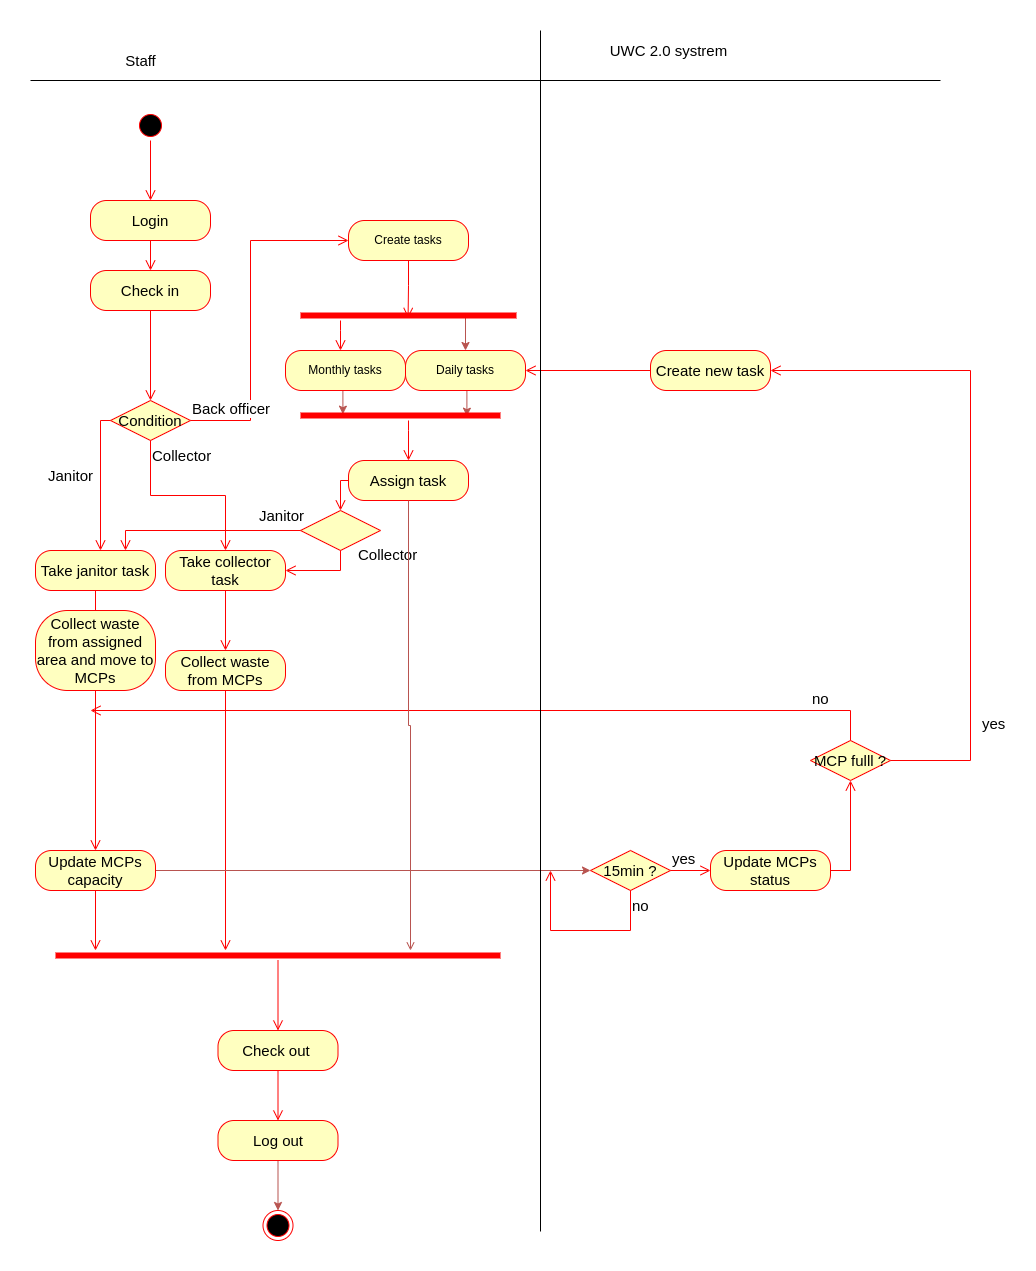
\includegraphics[scale=0.4]{system-modeling/diagramActivity.png}
        \caption{Activity Diagram}
        \label{fig:my_label}
    \end{figure}
\begin{tcolorbox}[colback=blue!5!white,colframe=blue!75!black]
The activity Diagram describes how activities are coordinated to provide a service which can be at different levels of abstraction. It is simply an advanced version of a flow chart that models the flow from one activity to another. The activity diagram above captures the dynamic behavior of the business process between systems and the stakeholders in the Task Assignment module which are back-officers, collectors and janitors. This diagram helps you understand the role of each stakeholder in the business and visualize the system model easier.
\end{tcolorbox}
\newpage
\subsection{Sequence Diagram}

\begin{center}
    \begin{figure}[!ht]
        \centering
        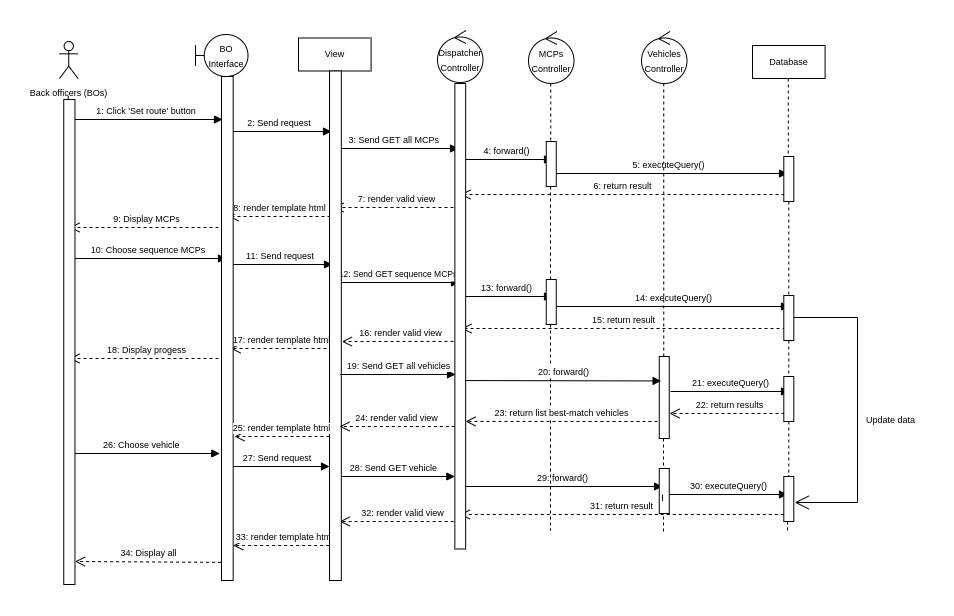
\includegraphics[scale=0.5]{system-modeling/diagramSequence.png}
        \caption{Sequence Diagram of Task Assignment Module}
        \label{fig:my_label}
    \end{figure}
\end{center}
\begin{tcolorbox}[colback=blue!5!white,colframe=blue!75!black]
For the Route planning task, our team proposed the following solution:
BO sends a request to the system to "Set route", and the system returns a list of available MCPs, BO then choose the available MCPs, and the system suggests the suitable vehicles based on the capacity and fuel consumption in regard to the chosen route, BO then selects the desirable vehicle, the system finally logs all the inputs of BO into the database. In our design, we are constructing an algorithm to calculate the suitable vehicles, taking into consideration the specifications of the vehicle and the features of the selected route. The system should be able to interact with the database to retrieve the wanted information and be able to perform the algorithm on said data to output the applicable selection of vehicles for the BO. In addition, we believed that the BO should be able to have flexibility in selecting the appropriate vehicle in case of any external factor, therefore, the BO will be given other options than the most viable.
\end{tcolorbox}
\newpage
\subsection{Class Diagram}

    \begin{figure}[!ht]
        \centering
        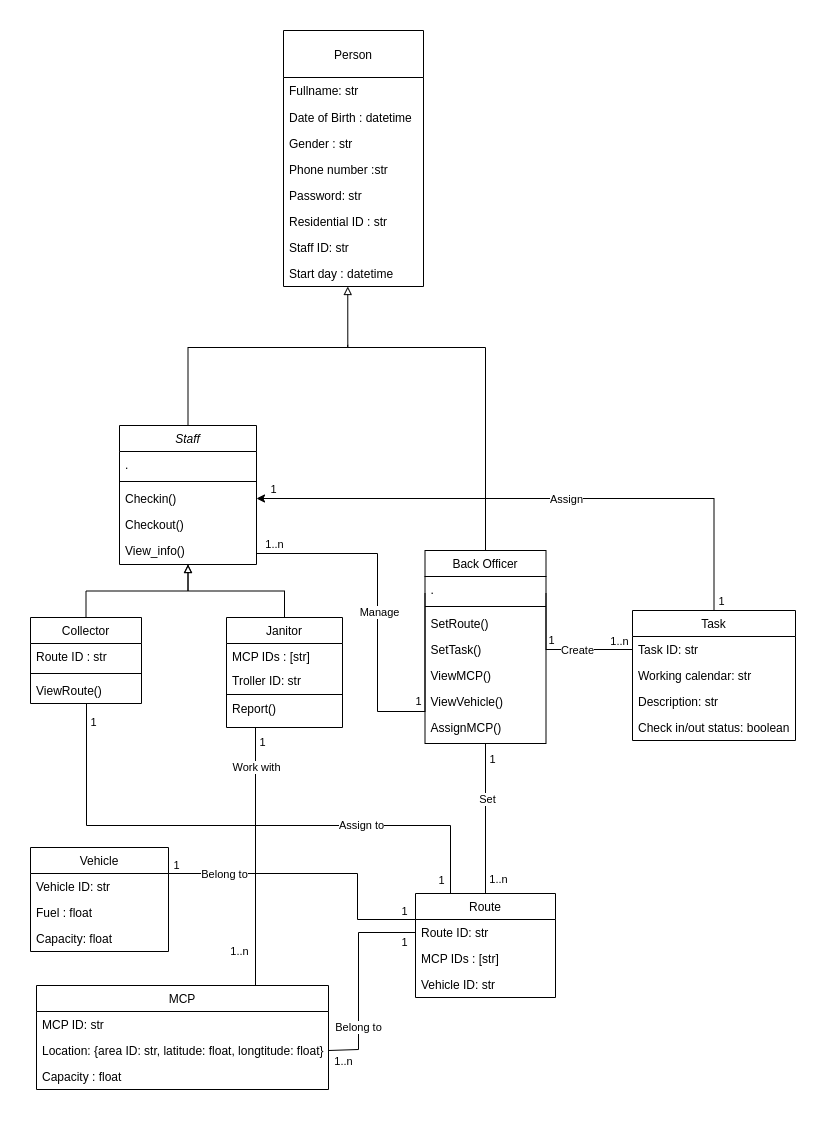
\includegraphics[scale=0.45]{system-modeling/diagramClass.png}
        \caption{Class Diagram}
        \label{fig:my_label}
    \end{figure}
    \begin{tcolorbox}[colback=blue!5!white,colframe=blue!75!black]
The class diagram describes the system models and data schema; it helps us visualize the system construct, its stakeholders, the models' relationship and how these models interact with each other in the system during the business process. To structure this diagram, we start with the personal information of each stakeholder. From the person class containing all information we need for an employee, we divided into different classes distinguished by their activities using inherent relationships. The diagram ends with classes defining labour tools that correspond with their stakeholders. 
\end{tcolorbox}

\newpage
\section{TASK\#3}
\subsection{Architectural approach of the system}
\subsubsection*{MVC Diagram}
\begin{figure}[!ht]
        \centering
        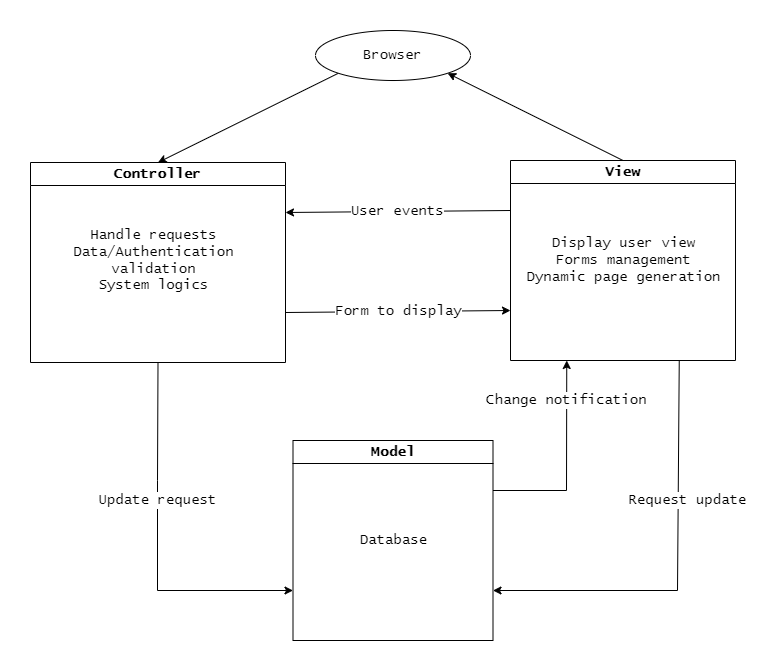
\includegraphics[scale=0.5]{architecture-design/diagramMVC.png}
        \caption{MVC Diagram}
        \label{fig:my_label}
    \end{figure}
\newpage
\subsubsection*{Description}
\begin{longtable}{|p{0.4\textwidth}|p{0.6\textwidth}|} 
    
         \multicolumn{2}{c}{} \\
         \hline 
         \endfirsthead
         
         \hline
        \caption{Specifying MVC diagram} \\
         \endlastfoot

         \hline
         \multicolumn{2}{l}{Continued from the previous page.}
         \hline
          
          \endhead

          \hline
         \multicolumn2{r}{Continued on the next page \ldots}\\
         \hline
        \endfoot

        \rowcolor{moccasin} \textbf{Name}  & \textbf{Description}  \\
        \hline 
        \textbf{Model}       &   Contains APIs for application-specific logics.  \\ 
                    &   Provides access to database management system for modifications  \\ 
                    &   Send refresh and update requests to View module when changes in Model module is detected  
                    
                    \hline
        \textbf{View}        &  Render user-specific views \\ 
                    &  Render drop-down menu and sliders when needed \\
                    &  Send user events to the Controller module \\
                    &  Update user input \\
                    &  Update UI when requested 
                    
                    \hline
        \textbf{Controller}  &  Return the appropriate view  \\
                    &  Data validation \\
                    &  Response to user events \\
       
\end{longtable} 
\subsection{Implementation Diagram}
\subsubsection*{Package Diagram}
\begin{figure}[H]
        \centering
        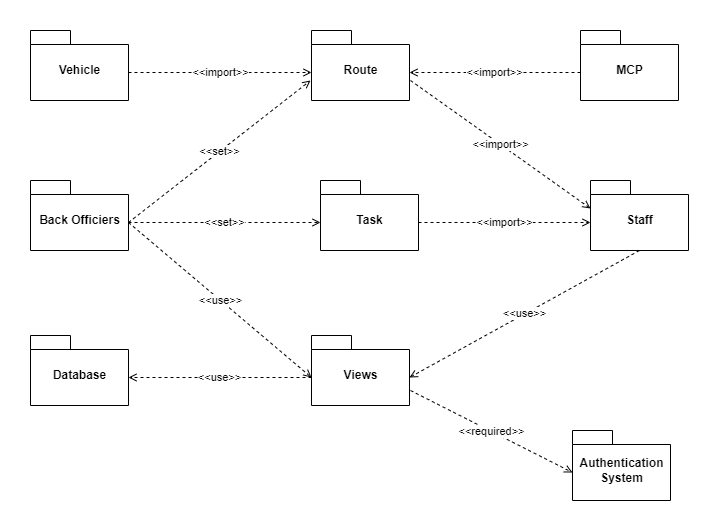
\includegraphics[scale=0.5]{architecture-design/diagramPackage.png}
        \caption{Package Diagram}
        \label{fig:my_label}
    \end{figure}\\
    \begin{tcolorbox}[colback=blue!5!white,colframe=blue!75!black]
We used a package diagram to simplify the complex class diagram, and organize the classes into packages. Therefore, we can visualize the whole system in a high-level abstraction. 
\end{tcolorbox}
\subsubsection*{Component Diagram}
\begin{figure}[H]
        \centering
        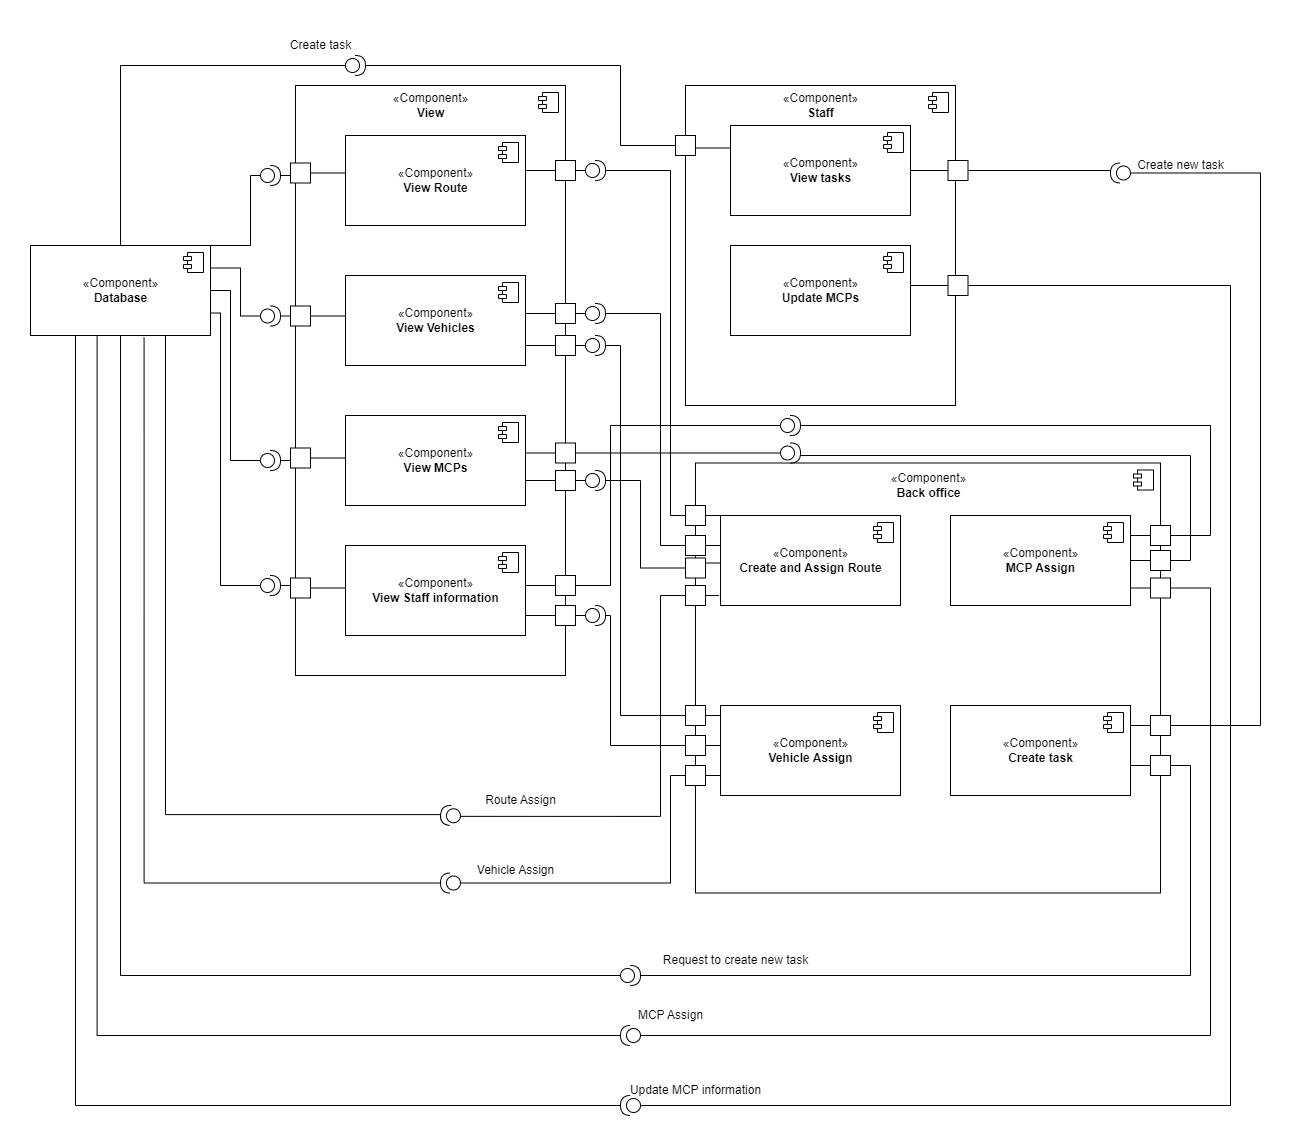
\includegraphics[scale=0.35]{architecture-design/diagramComponent.png}
        \caption{Component Diagram}
        \label{fig:my_label}
\end{figure}
\begin{tcolorbox}[colback=blue!5!white,colframe=blue!75!black]

In terms of component diagram, we describe 5 components including staff, back officer, view, database, and authentication. Actually, the authenticate process is compulsory before using services, thus, one can assume that interactions between actors (such as staffs or back officers) and services of the system have involved successful authentication. We represent each component in the following sections.
\end{tcolorbox}
%
\subsection{Modules}
In our design, we propose the following breakdown structure includes three main modules:
\subsubsection*{Task Assignment}
In this modules, the back officers create and assign tasks for collectors and janitors, provided all necessary allocated resources such as MCPs, specification of vehicles, etc. 
\begin{itemize}
    \item Input:
    \begin{itemize}
        \item MCPs
        \item Vehicles
        \item Collectors
        \item Janitors
    \end{itemize}
    \item Output:
    \begin{itemize}
        \item Tasks (assigned to 
        \item Routes (assigned to 
    \end{itemize}
\end{itemize}
\subsubsection*{Authentication}
In this module, the system handles authentication requests, including but not limited to log in, log out, registration, etc.
\begin{itemize}
    \item Input:
    \begin{itemize}
        \item Staff ID
        \item Password
        \item Personal information
    \end{itemize}
    \item Output:
    \begin{itemize}
        \item Access token
        \item Account's information
    \end{itemize}
\end{itemize}
\subsubsection*{Display}
In this module, the system renders the appropriate view for each users, handles requests from client devices.
\begin{itemize}
    \item Output:
    \begin{itemize}
        \item Route
        \item Task's dashboard
        \item Account's information
    \end{itemize}
\end{itemize}

\section{Revision versions}
\texttt{To be determined...}
    
\centering --END--
\end{document}
